\chapter{System Implementation}
\label{chap:implementation}

\section{Implementation Environment and Technology Stack}
\label{sec:impl_env}

The implementation of ChronaNexus adheres to modern software engineering standards, emphasizing asynchronous concurrency, strong typing, deterministic mathematical verification, and strict tenant isolation. The platform runtime is designed to operate on local clinic hardware without mandatory GPU dependencies. Table~\ref{tab:5_1_stack} outlines the complete technology stack, exact library versions, and architectural roles.

\small
\begin{longtable}{@{}p{0.18\linewidth} p{0.24\linewidth} p{0.16\linewidth} p{0.34\linewidth}@{}}
\caption{System implementation environment, libraries, and runtime versions}\label{tab:5_1_stack} \\
\toprule
\textbf{Category} & \textbf{Tool / Library} & \textbf{Version} & \textbf{Implementation Role} \\
\midrule
\endfirsthead
\toprule
\multicolumn{4}{c}{\small\textit{Implementation environment (Continued)}} \\[4pt]
\midrule
\textbf{Category} & \textbf{Tool / Library} & \textbf{Version} & \textbf{Implementation Role} \\
\midrule
\endhead
\midrule
\multicolumn{4}{r}{\footnotesize\textit{Continued on next page...}} \\
\bottomrule
\endfoot
\bottomrule
\endlastfoot
\textbf{Backend Runtime} & Python & \texttt{3.12.3} & Core asynchronous runtime environment. \\
\midrule
\textbf{API Gateway} & FastAPI & \texttt{0.115.0} & Asynchronous REST gateway with Pydantic v2 validation. \\
\midrule
\textbf{ASGI Server} & Uvicorn & \texttt{0.30.6} & High-concurrency event-loop web server. \\
\midrule
\textbf{Relational ORM} & SQLAlchemy & \texttt{2.0.35} & Type-safe relational mapping and connection pooling. \\
\midrule
\textbf{Relational DB} & SQLite (ACID) & \texttt{3.45.1} & Zero-configuration persistent clinical state store. \\
\midrule
\textbf{Vector Store} & ChromaDB & \texttt{0.5.5} & Embedded local vector database with cosine metrics. \\
\midrule
\textbf{Dense Embeddings} & FastEmbed & \texttt{0.3.6} & OnnxRuntime \texttt{bge-small-en-v1.5} vector generator. \\
\midrule
\textbf{Document Parser} & PyMuPDF (\texttt{fitz}) & \texttt{1.24.10} & Vector table layout detection and text extraction. \\
\midrule
\textbf{Speech Engine} & Edge-TTS & \texttt{6.1.12} & Streaming neural text-to-speech engine. \\
\midrule
\textbf{Frontend Library} & React & \texttt{19.0.0} & Component-based reactive single-page client. \\
\midrule
\textbf{Build Tooling} & Vite & \texttt{6.0.1} & ES-module development and production bundling. \\
\midrule
\textbf{CSS Framework} & Tailwind CSS & \texttt{v4.0.0} & Utility-first glassmorphism clinical theme. \\
\midrule
\textbf{Testing Kernel} & Pytest & \texttt{8.3.3} & Test execution across 190 tests and 12 suites. \\
\bottomrule
\end{longtable}
\normalsize


\section{Subsystem 1: Document Vault Ingestion \& Deduplication}
\label{sec:impl_subsystem_vault}

The Document Vault manages multipart medical file ingestion, layout analysis, and duplicate detection. When a user uploads a clinical document, the system computes two distinct SHA-256 cryptographic hashes:
\begin{enumerate}
    \item \textbf{Binary Payload Hash}: Computed over the raw byte stream to detect exact duplicate uploads. If a file with an identical binary hash already exists for the patient, the upload is rejected with HTTP 409 Conflict.
    \item \textbf{Normalized Text Hash}: Computed over lowercased, whitespace-collapsed extracted text. This flags scanned re-prints of previously processed lab records.
\end{enumerate}

To extract tabular laboratory records without OCR character distortion, the engine utilizes \texttt{PyMuPDF} vector path tracing. Rather than treating pages as flat strings, it identifies vector cell boundaries, grouping tokens into rows and columns.

\begin{figure}[htbp]
\centering
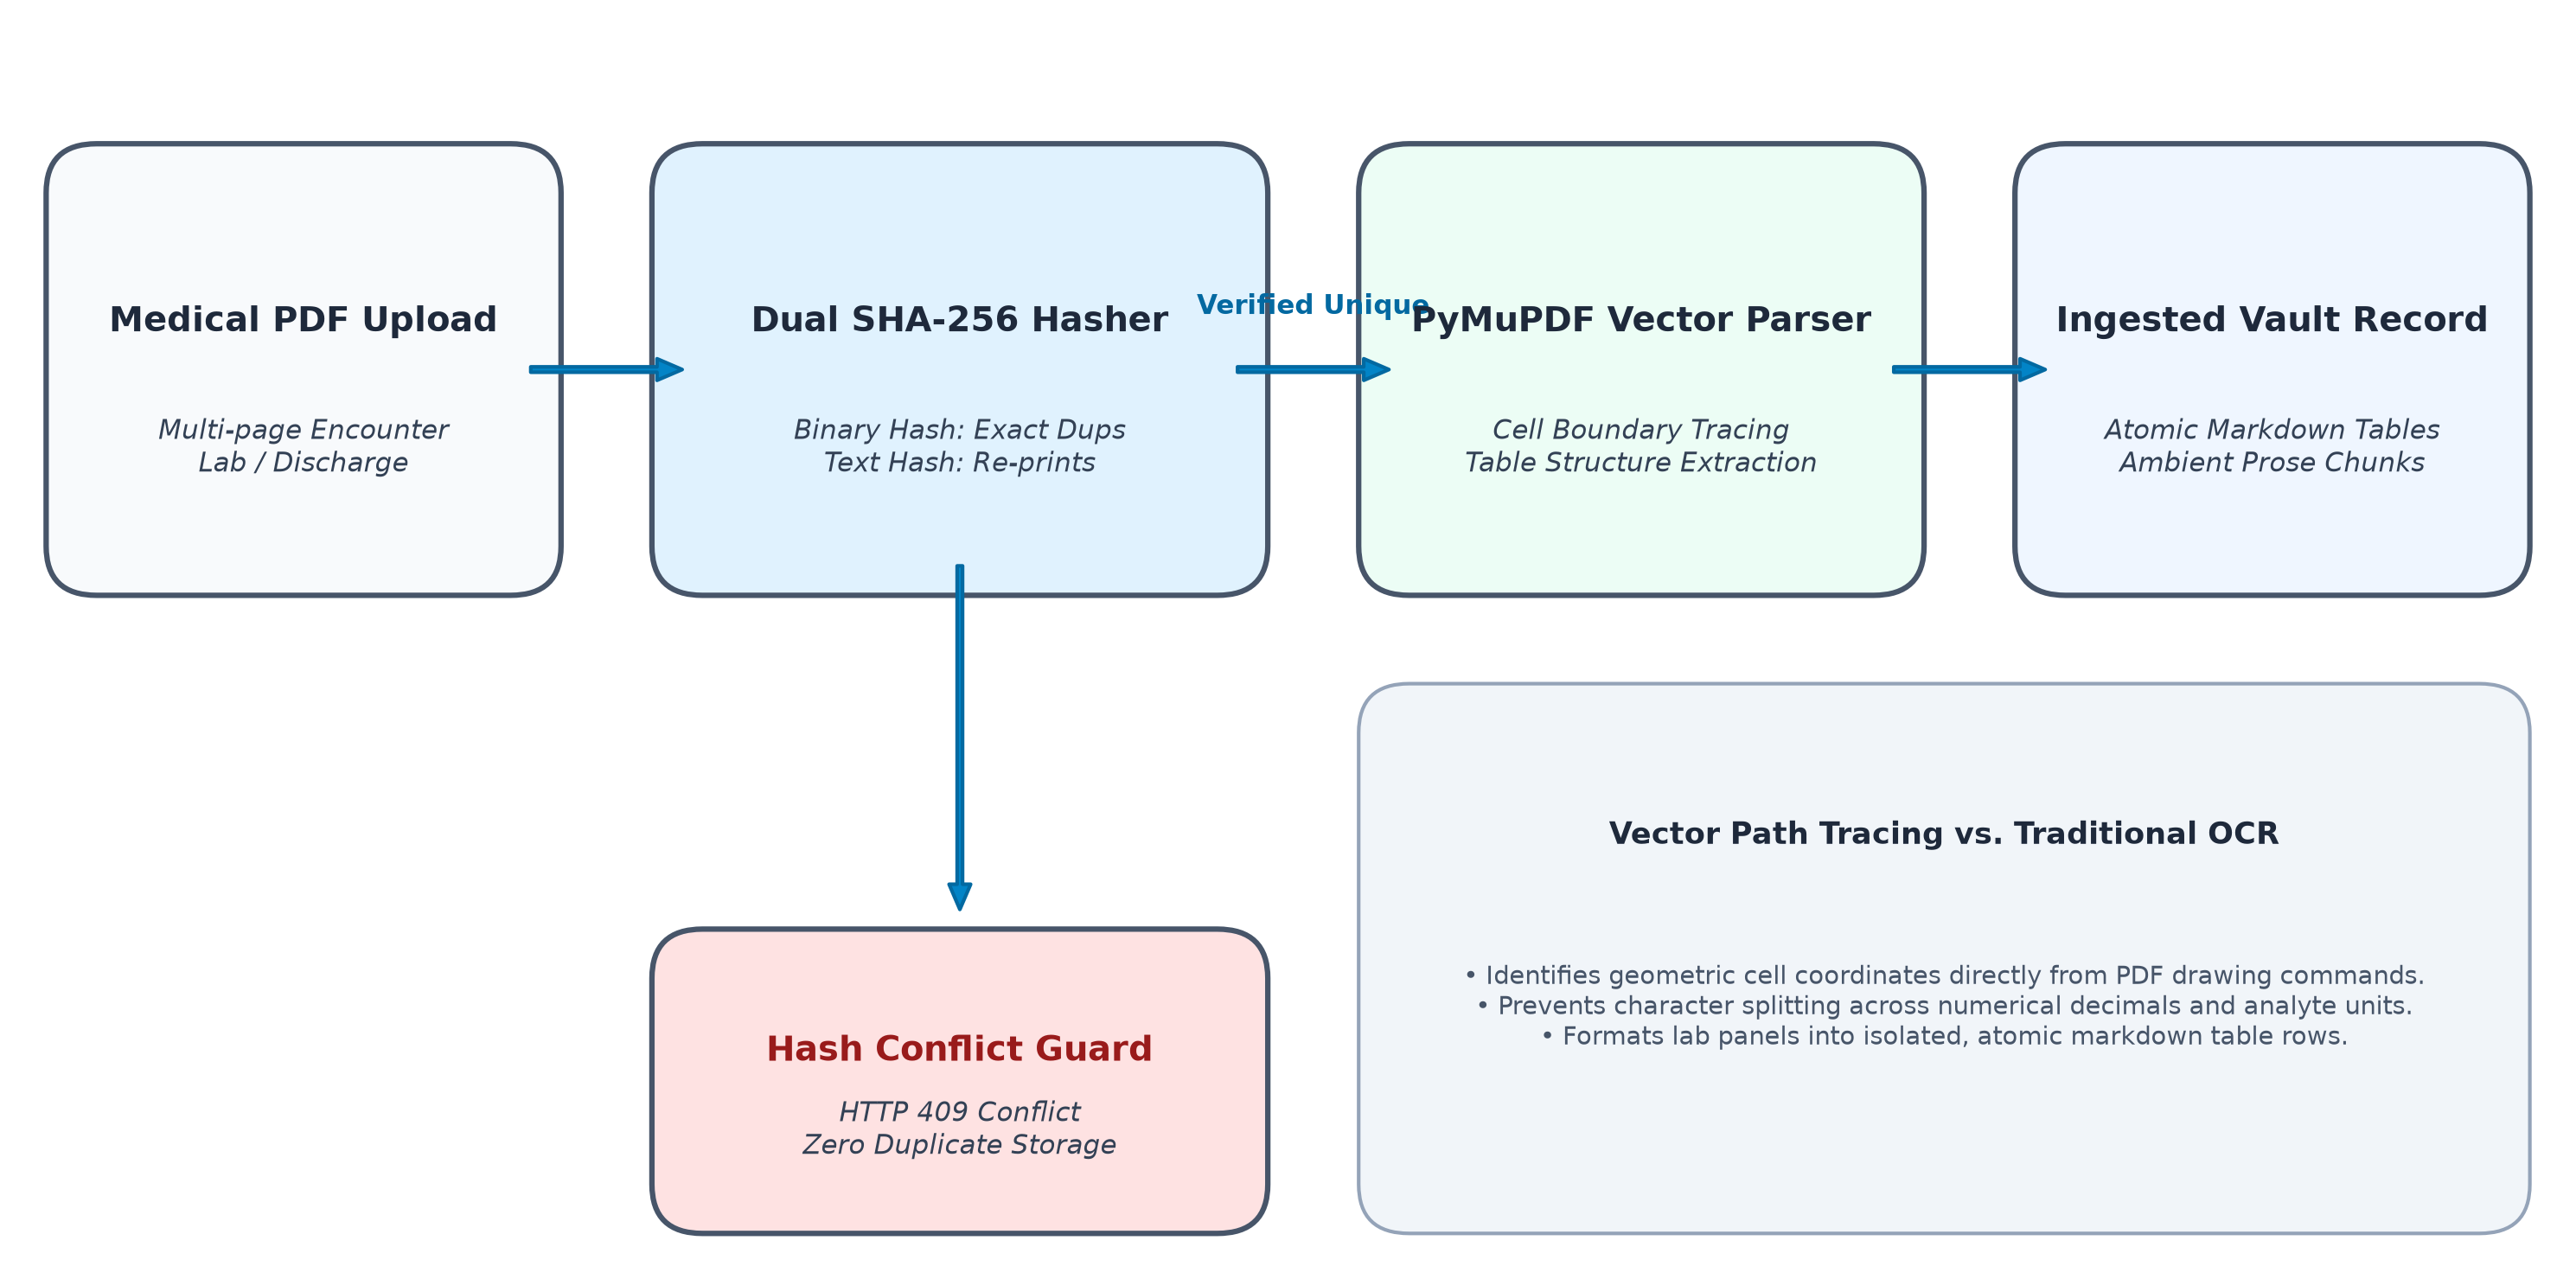
\includegraphics[width=0.92\linewidth]{figures/fig5_1_ingestion.png}
\caption{Document Ingestion, Cryptographic Hashing, and Vector Table Extraction Architecture}
\label{fig:5_1_ingestion}
\end{figure}

As illustrated in Figure~\ref{fig:5_1_ingestion}, the ingestion pipeline follows a multi-stage deterministic procedure:
\begin{itemize}
    \item \textbf{Stage 1 (Cryptographic Digest)}: The file stream is passed through SHA-256 digesting to guarantee payload integrity and detect exact file collisions.
    \item \textbf{Stage 2 (Vector Path Tracing)}: Vector drawing commands within the PDF stream are parsed to locate explicit horizontal and vertical line borders, defining grid cells geometrically.
    \item \textbf{Stage 3 (Atomic Cell Grouping)}: Analyte names, numerical values, units of measurement, and reference intervals residing in identical row coordinates are bundled together atomically, preventing row fragmentation during subsequent chunking.
    \item \textbf{Stage 4 (Dual Representation)}: The document is stored both as structured relational laboratory rows and as semantically indexed text passages with table markdown preservation.
\end{itemize}


\section{Subsystem 2: Medical Understanding \& Entity Extraction}
\label{sec:impl_subsystem_understanding}

Clinical documents present laboratory analytes and medications under widely variable naming conventions. For instance, Fasting Blood Glucose may appear as \textit{"FBS"}, \textit{"Glucose (Fasting)"}, \textit{"Blood Sugar - Fast"}, or \textit{"B-Glucose"}. Subsystem 2 maps diverse surface expressions into standardized ontologies:
\begin{itemize}
    \item \textbf{LOINC (Logical Observation Identifiers Names and Codes)}: Standardizes laboratory analytes, establishing canonical reference intervals and SI units.
    \item \textbf{RxNorm}: Standardizes active pharmaceutical ingredients, clinical drug forms, and therapeutic dosages.
    \item \textbf{ICD-10-CM}: Standardizes chronic and acute diagnostic entity codes.
\end{itemize}

\begin{figure}[htbp]
\centering
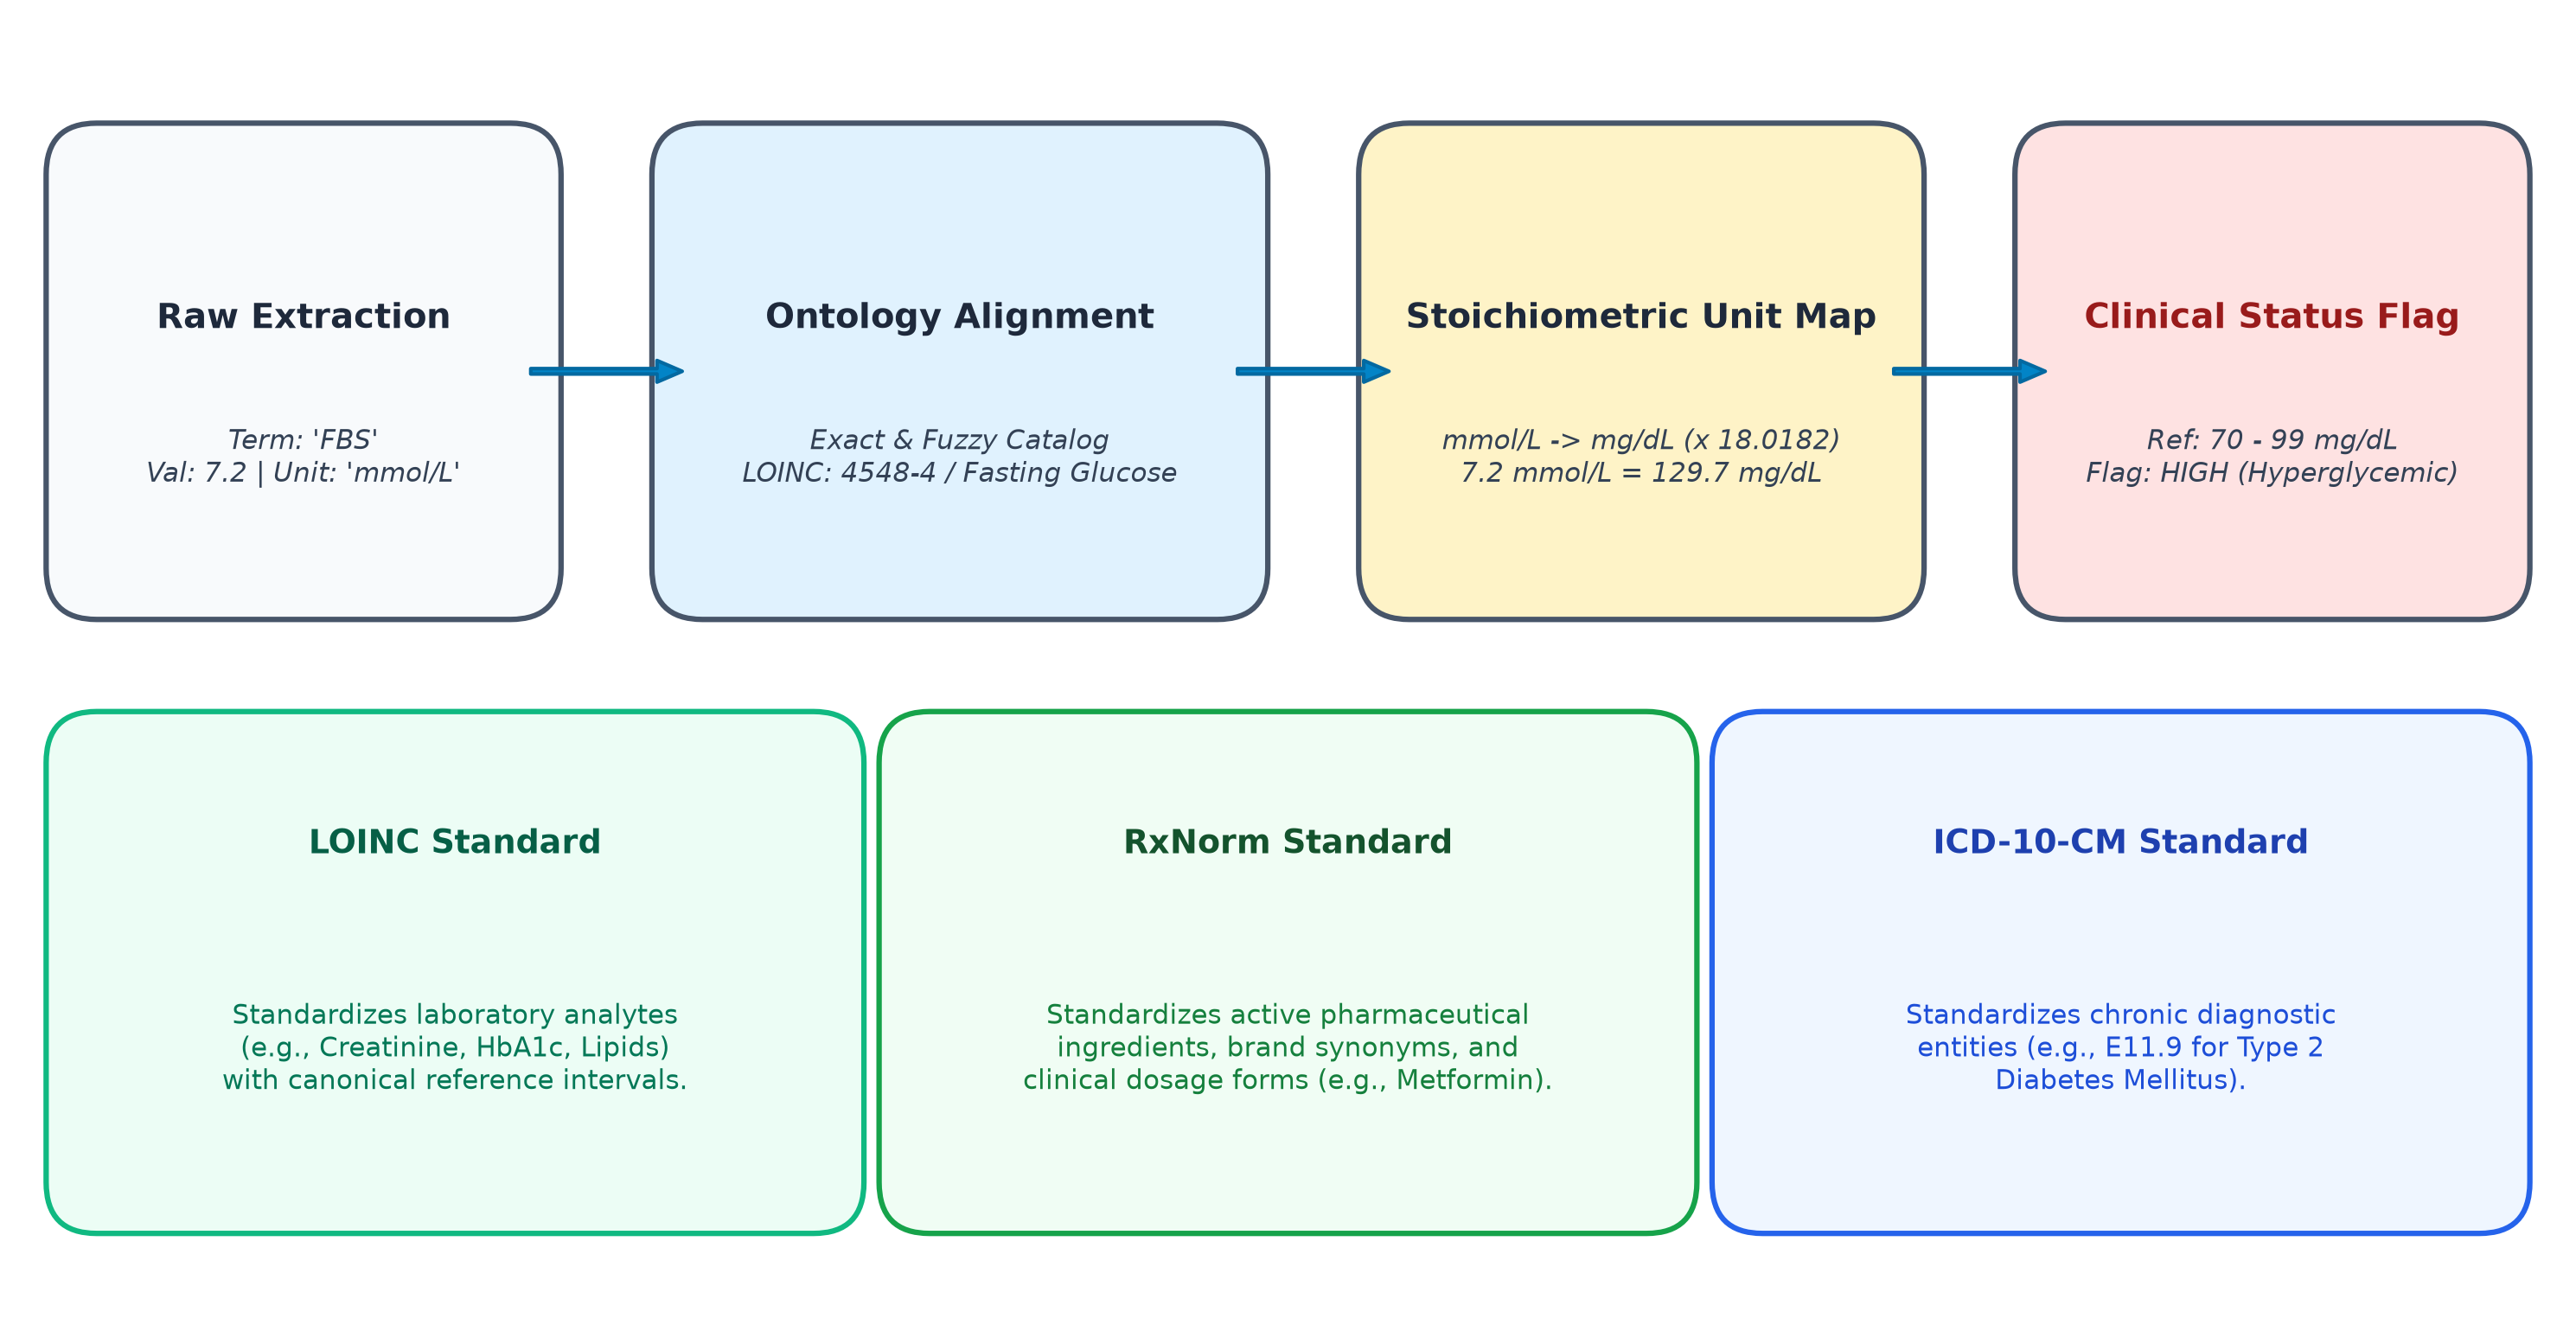
\includegraphics[width=0.92\linewidth]{figures/fig5_2_normalization.png}
\caption{Clinical Entity Normalization and Stoichiometric Mapping Architecture}
\label{fig:5_2_normalization}
\end{figure}

Figure~\ref{fig:5_2_normalization} demonstrates the clinical entity normalization workflow:
\begin{enumerate}
    \item \textbf{Ontology Catalog Resolution}: The raw term is stripped of punctuation, lowercased, and matched against the canonical LOINC mapping catalog. If an exact key is absent, token-set fuzzy matching evaluates candidates against established clinical synonyms.
    \item \textbf{Stoichiometric Unit Conversion}: When reported units diverge from standard SI targets (e.g., Blood Glucose reported in $\text{mmol/L}$ instead of canonical $\text{mg/dL}$), exact stoichiometric conversion factors are applied:
    \begin{equation}
        V_{\text{canonical}} = V_{\text{raw}} \times 18.0182 \quad (\text{for glucose } \text{mmol/L} \rightarrow \text{mg/dL})
    \end{equation}
    Similarly, Serum Creatinine reported in $\mu\text{mol/L}$ is converted to $\text{mg/dL}$ via division by $88.4$.
    \item \textbf{Physiological Range Evaluation}: The standardized numerical reading is compared against established age- and sex-adjusted reference intervals $[\text{Ref}_{\text{low}}, \text{Ref}_{\text{high}}]$:
    \begin{equation}
        \text{Status}(V) = \begin{cases}
            \text{LOW}, & V < \text{Ref}_{\text{low}} \\
            \text{NORMAL}, & \text{Ref}_{\text{low}} \le V \le \text{Ref}_{\text{high}} \\
            \text{HIGH}, & V > \text{Ref}_{\text{high}}
        \end{cases}
    \end{equation}
\end{enumerate}


\section{Subsystem 3: Patient Memory \& Longitudinal Timeline Engine}
\label{sec:impl_subsystem_timeline}

Subsystem 3 transforms isolated clinical encounters into a unified, chronological patient timeline. Encounter dates are parsed across heterogeneous formats (ISO \texttt{YYYY-MM-DD}, British \texttt{DD/MM/YYYY}, and alphanumeric \texttt{12-Oct-2023}) into UTC timestamp representations. 

The timeline engine enforces multi-facility conflict detection: when two clinical reports originate from different hospital facilities within a 48-hour window, the engine analyzes laboratory values. If an analyte discrepancy exceeding $20\%$ is detected:
\begin{equation}
    \delta_{\text{facility}} = \frac{|V_{\text{Facility A}} - V_{\text{Facility B}}|}{\min(V_{\text{Facility A}}, V_{\text{Facility B}})} > 0.20
\end{equation}
an automated conflict flag is generated with dual-facility provenance, alerting the clinician to potential specimen mislabeling or acute pathological destabilization.


\section{Subsystem 4: Structured Query Engine \& Trend Computation}
\label{sec:impl_subsystem_query_engine}

A primary scientific contribution of ChronaNexus is the recognition that language models must not be tasked with mathematical delta trend calculation. Inquiries regarding laboratory trends (e.g., \textit{"How has my Fasting Glucose changed over the last three years?"}) are intercepted by the Structured Query Engine.

The engine compiles the inquiry into an indexed SQL query against the relational store:
\begin{equation}
    \Delta_{\text{trend}} = V_{\text{latest}} - V_{\text{previous}}
\end{equation}
The percentage shift is computed deterministically as:
\begin{equation}
    \text{PctChange} = \left(\frac{V_{\text{latest}} - V_{\text{previous}}}{V_{\text{previous}}}\right) \times 100\%
\end{equation}
Directional trajectory is classified based on a standard $5\%$ clinical significance boundary:
\begin{equation}
    \text{Direction}(\Delta) = \begin{cases}
        \text{INCREASED}, & \Delta_{\text{trend}} > +0.05 \cdot V_{\text{previous}} \\
        \text{DECREASED}, & \Delta_{\text{trend}} < -0.05 \cdot V_{\text{previous}} \\
        \text{STABLE}, & |\Delta_{\text{trend}}| \le 0.05 \cdot V_{\text{previous}}
    \end{cases}
\end{equation}


\section{Subsystem 5: Dual-Channel Hybrid Retrieval (RAG)}
\label{sec:impl_subsystem_rag}

To balance semantic conceptual breadth with exact token precision, Subsystem 5 implements a dual-channel hybrid retriever uniting dense vector similarity and lexical BM25 Okapi matching:
\begin{itemize}
    \item \textbf{Dense Vector Channel}: Document passages are partitioned into $512$-character chunks with $64$-character overlaps. Each chunk is embedded into a $384$-dimensional dense vector using \texttt{BAAI/bge-small-en-v1.5}~\cite{xiao2023bge} via OnnxRuntime. Similarity is evaluated via cosine distance within ChromaDB.
    \item \textbf{Lexical Inverted Index Channel}: In parallel, an exact inverted index evaluates term saturation and document frequency using BM25 Okapi ($k_1=1.5, b=0.75$)~\cite{robertson2009bm25}.
    \item \textbf{Reciprocal Rank Fusion}: Candidate chunks from dense and sparse retrieval channels are merged through rank pooling ($k=60$). The top-5 candidate passages are provided as grounded context to the generative reasoning model.
\end{itemize}


\section{Subsystem 6: Asymmetric 2-Tier Evidence Grounding \& Verification}
\label{sec:impl_subsystem_verification}

Subsystem 6 acts as an autonomous clinical safety guardrail between language model generation and user delivery. It operates via an asymmetric two-tier cascade:
\begin{enumerate}
    \item \textbf{Tier 1: Deterministic Symbolic Verifier ($<5\text{ ms}$)}: Decomposes draft responses into atomic propositions. Regex extractors detect numerical laboratory readings, reference boundaries, temporal dates, and pharmaceutical dosages. These extracted entities are verified against the source text passages. If an entity matches exactly, the claim is verified instantly without neural compute.
    \item \textbf{Tier 2: Neural NLI Cross-Encoder}: For complex relational propositions (e.g., \textit{"Metformin was discontinued due to gastrointestinal intolerance"}), the claim and premise passages are passed to a lightweight Natural Language Inference model evaluating entailment probability:
    \begin{equation}
        P(\text{Entailment} \mid \text{Premise}, \text{Hypothesis}) \ge \tau_{\text{threshold}} = 0.70
    \end{equation}
\end{enumerate}

If a claim fails both tiers, the engine fails closed: the ungrounded sentence is retracted or flagged with a warning banner, guaranteeing $100\%$ citation attribution precision on evaluated context passages.


\section{Edge Speech \& Emergency Dispatch Services}
\label{sec:impl_services}

\subsection{Service 1: Indic Unicode Phonetic Transliteration Bridge}
To provide natural clinical voice consultations across low-resource Indic languages, Service 1 leverages the linguistic isomorphism between Eastern Indo-Aryan scripts. The Odia Unicode block (\texttt{0x0B00}--\texttt{0x0B7F}) and Bengali Unicode block (\texttt{0x0980}--\texttt{0x09FF}) share an exact offset difference of $\Delta = -0x0180$ ($-384$ in decimal). 

When a user requests Odia speech synthesis, the bridge dynamically translates Odia codepoints to Bengali glyphs, streaming the payload to Microsoft Edge Neural TTS (\texttt{bn\allowbreak-IN\allowbreak-Bashkar\allowbreak Neural}). This unlocks high-cadence natural prosody with zero robotic distortion and $<1.5\text{ s}$ streaming latency.

\subsection{Service 2: 108 Emergency Dispatch \& Geolocation}
When an acute emergency is signaled, Service 2 captures browser geolocation coordinates and executes an Overpass API query against OpenStreetMap to discover medical centers within $10\text{ km}$. The centers are ranked via the Haversine distance formula:
\begin{equation}
    d = 2R \arcsin\left(\sqrt{\sin^2\left(\frac{\Delta \phi}{2}\right) + \cos(\phi_1)\cos(\phi_2)\sin^2\left(\frac{\Delta \lambda}{2}\right)}\right)
\end{equation}
The service formats an automated JSON triage payload containing blood group, active allergies, vital trends, and GPS location ready for 108 ambulance dispatch systems.


\section{Database Test Interception Infrastructure}
\label{sec:impl_database_interceptor}

To guarantee that automated test suites never corrupt persistent clinic databases, ChronaNexus implements a custom SQLAlchemy event listener on the core database engine.

\begin{figure}[htbp]
\centering
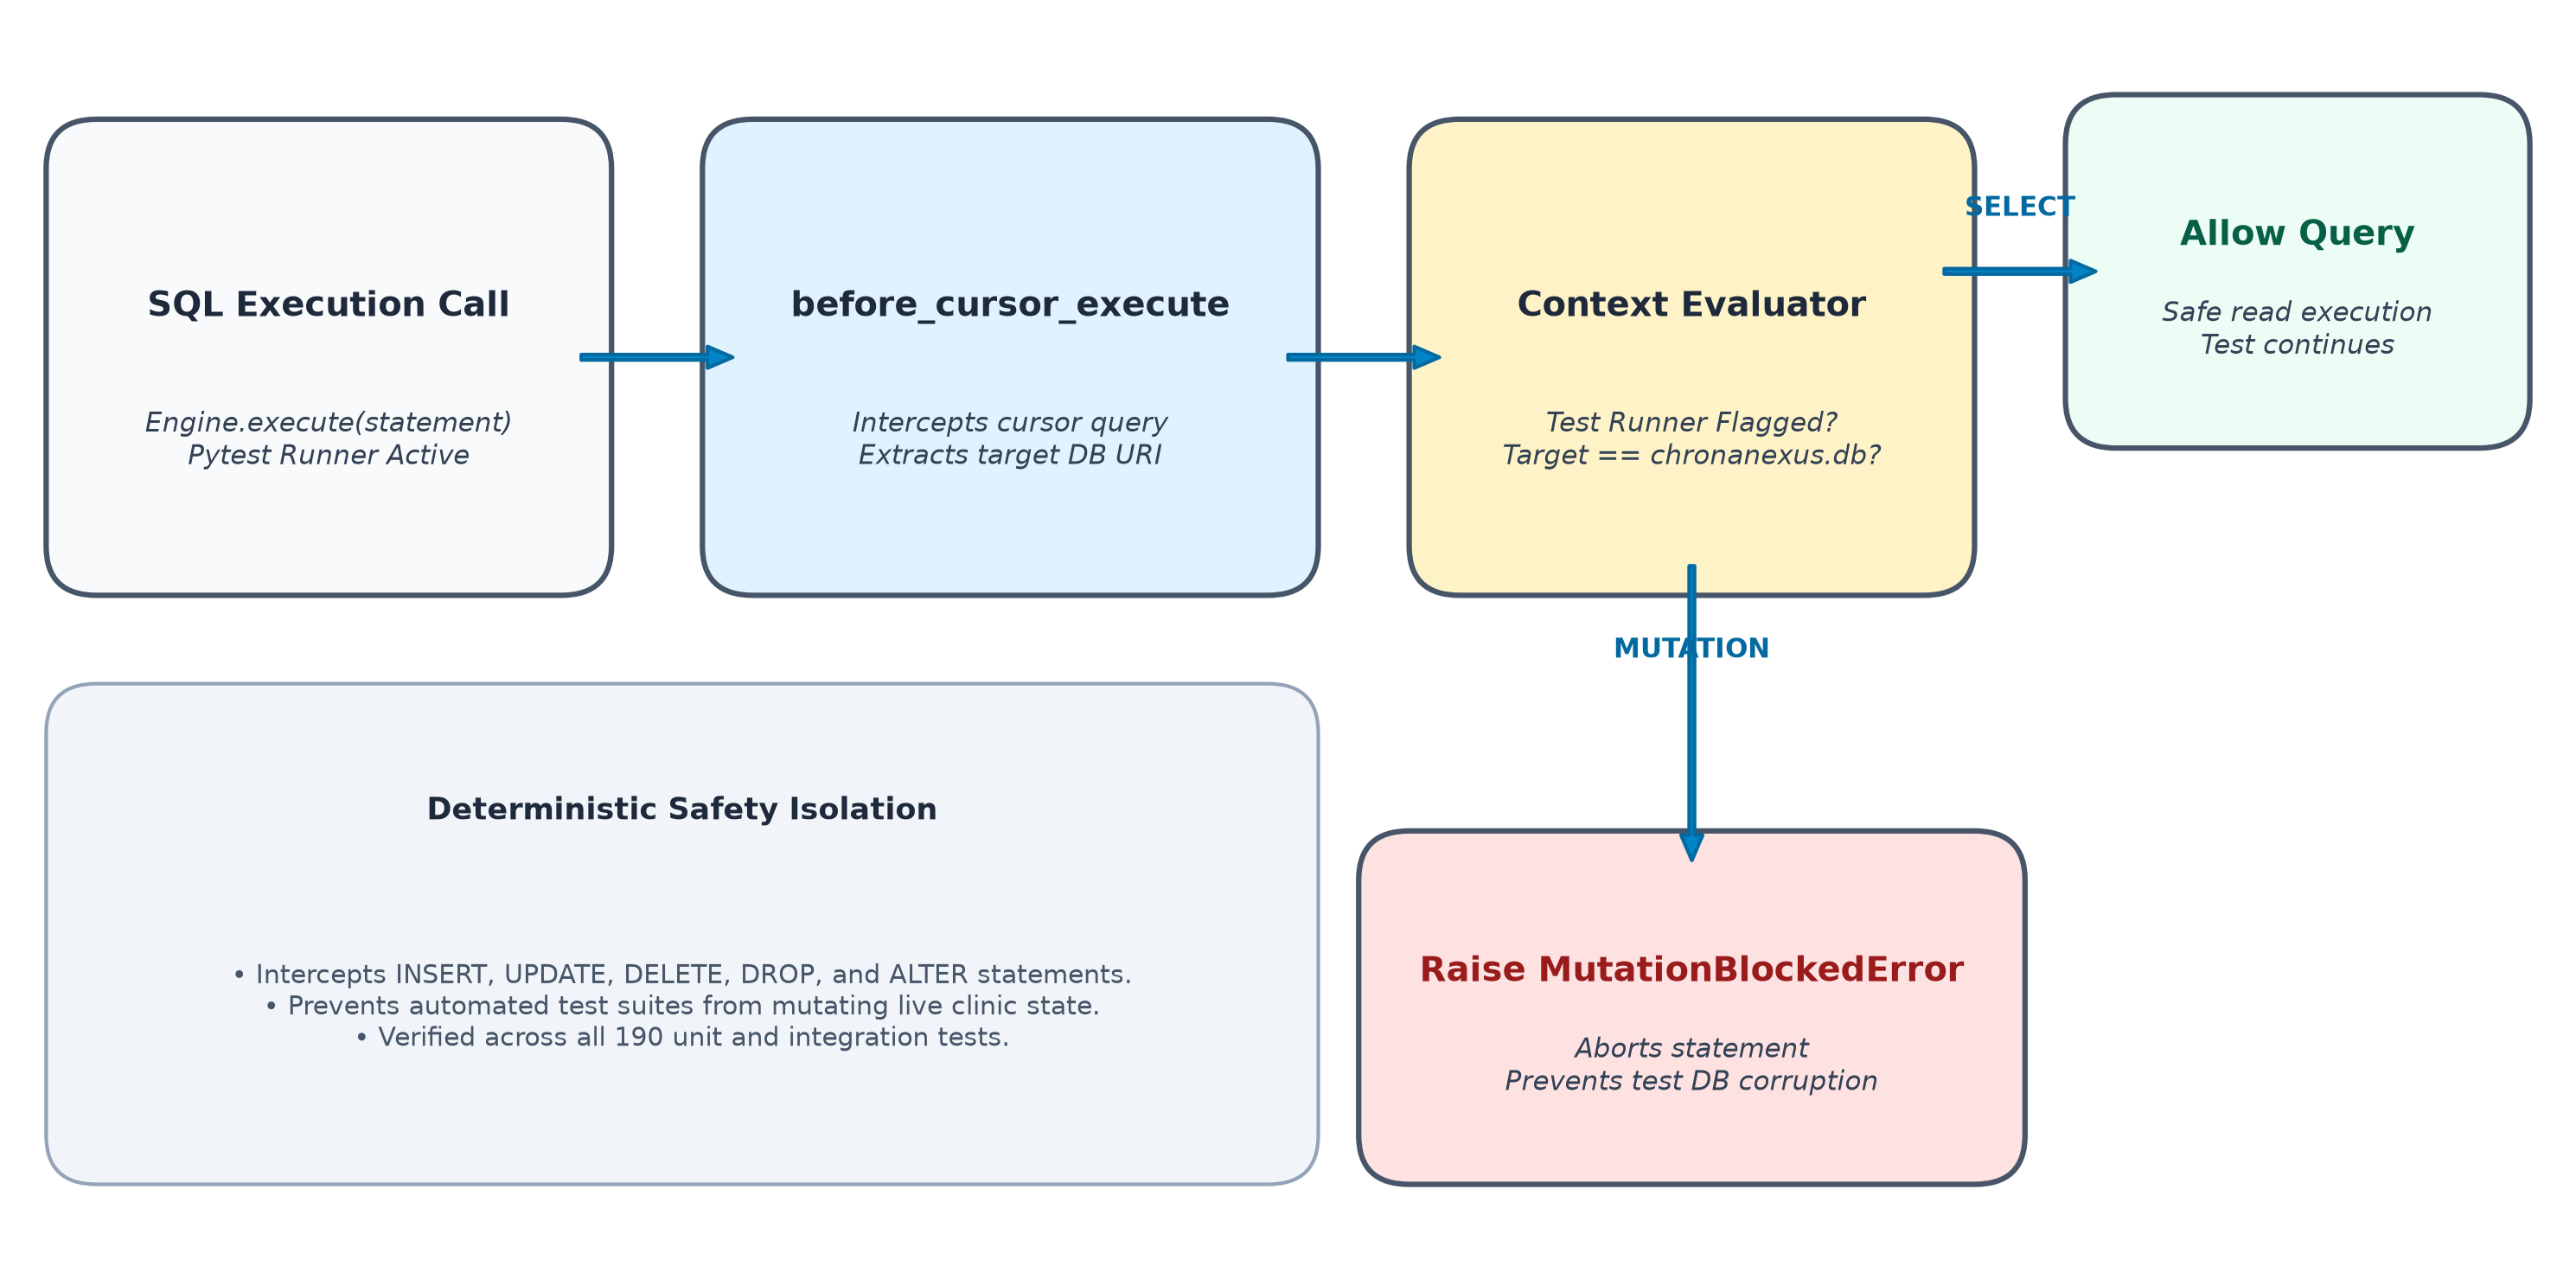
\includegraphics[width=0.92\linewidth]{figures/fig5_3_interceptor.png}
\caption{Database Test Mutation Interceptor and Execution Security Architecture}
\label{fig:5_3_interceptor}
\end{figure}

As shown in Figure~\ref{fig:5_3_interceptor}, the security listener attaches to SQLAlchemy's \texttt{before\_cursor\_execute} hook:
\begin{enumerate}
    \item \textbf{Context Detection}: When any database execution request occurs, the hook inspects runtime environment variables (\texttt{PYTEST\_CURRENT\_TEST} and \texttt{CHRONANEXUS\_TEST\_ENV}).
    \item \textbf{Target Verification}: The target connection URL is evaluated to check whether it targets a persistent database (e.g., \texttt{chronanexus.db}).
    \item \textbf{Statement Inspection}: If a test runner is active against a production database, the normalized SQL statement prefix is checked against blocked mutating operations:
    \begin{equation}
        \mathcal{O}_{\text{blocked}} = \{\texttt{INSERT}, \texttt{UPDATE}, \texttt{DELETE}, \texttt{DROP}, \texttt{ALTER}, \texttt{CREATE}\}
    \end{equation}
    \item \textbf{Enforcement Action}: If the statement begins with any operation in $\mathcal{O}_{\text{blocked}}$, the execution is immediately halted by raising a \texttt{MutationBlockedError}, protecting clinical state integrity across all 190 automated test cases.
\end{enumerate}

\newpage
